\clearpage
\subsection{Colour Test Runs} % (fold)
\label{sub:colour_tests}
Depending on which house the user belongs to, the system should theme itself in that house's colours.

\begin{figure}[!htbp]
\centering
\begin{subfigure}{0.5\textwidth}
  \centering
  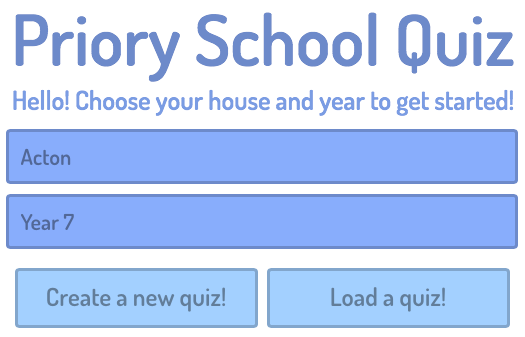
\includegraphics[width=0.95\linewidth]{testing/colours/acton}
  \caption{Acton}
  \label{fig:sub1}
\end{subfigure}%
\begin{subfigure}{0.5\textwidth}
  \centering
  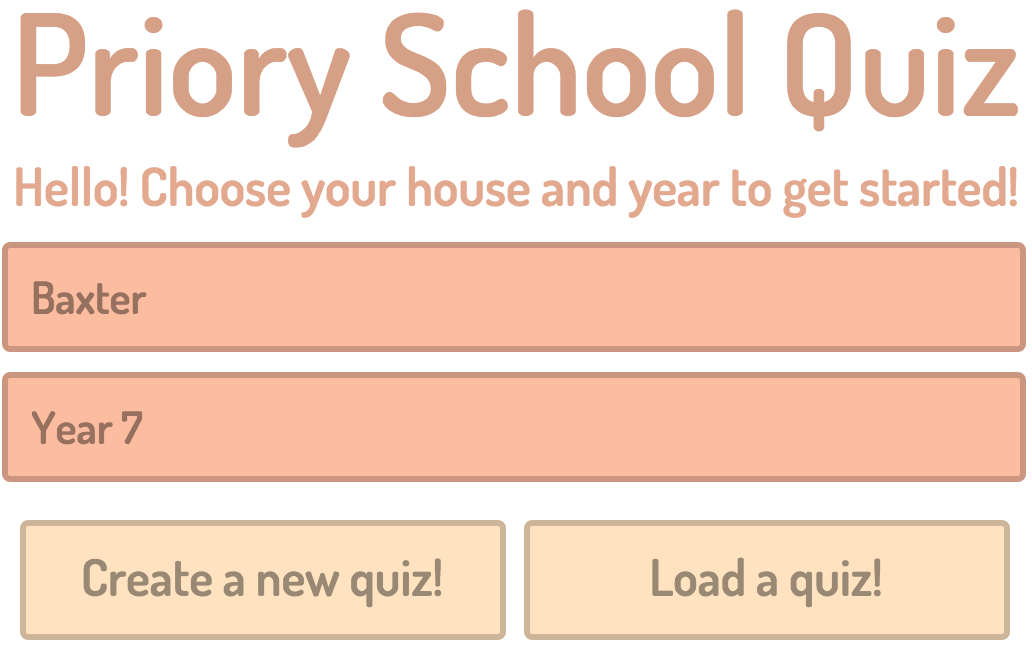
\includegraphics[width=0.95\linewidth]{testing/colours/baxter}
  \caption{Baxter}
  \label{fig:sub2}
\end{subfigure}
\label{fig:test}
\end{figure}

\begin{figure}[!htbp]
\centering
\begin{subfigure}{0.5\textwidth}
  \centering
  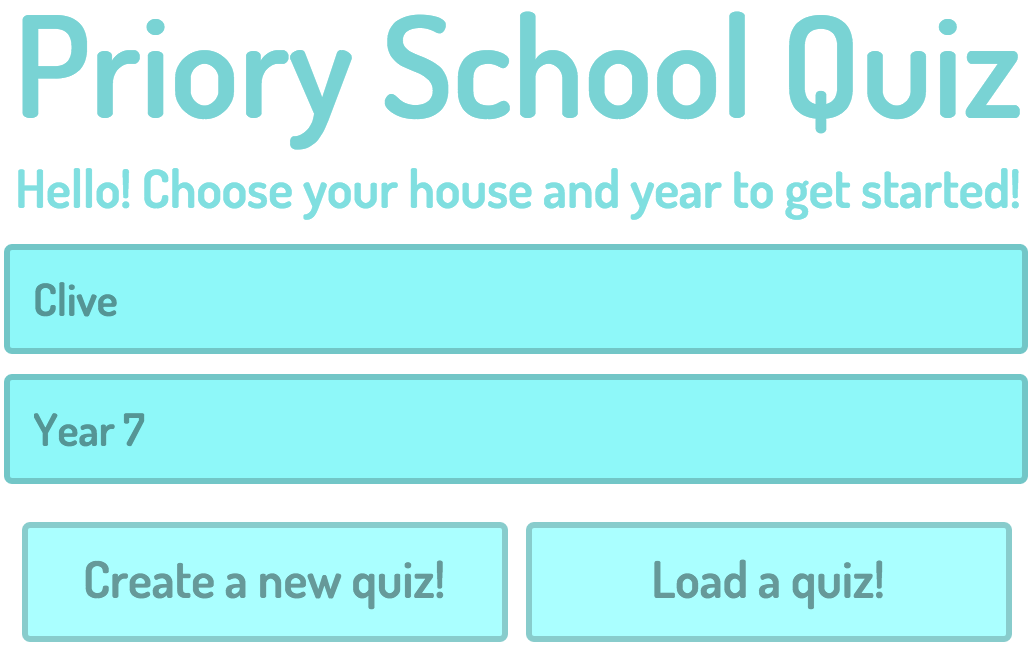
\includegraphics[width=0.95\linewidth]{testing/colours/clive}
  \setcounter{subfigure}{2}%
  \caption{Clive}
  \label{fig:sub1}
\end{subfigure}%
\begin{subfigure}{0.5\textwidth}
  \centering
  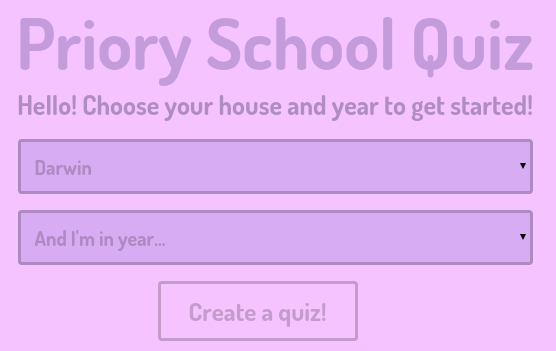
\includegraphics[width=0.95\linewidth]{testing/colours/darwin}
  \setcounter{subfigure}{3}%
  \caption{Darwin}
  \label{fig:sub2}
\end{subfigure}
\label{fig:test}
\end{figure}

\begin{figure}[!htbp]
\centering
\begin{subfigure}{0.5\textwidth}
  \centering
  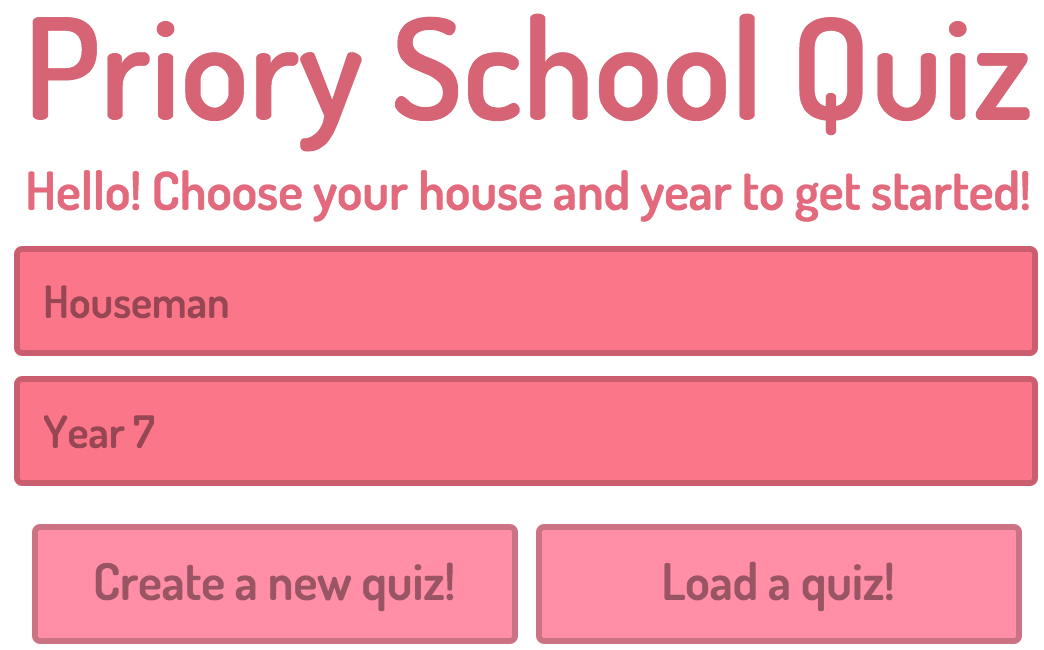
\includegraphics[width=0.95\linewidth]{testing/colours/houseman}
  \setcounter{subfigure}{4}%
  \caption{Houseman}
  \label{fig:sub1}
\end{subfigure}%
\begin{subfigure}{0.5\textwidth}
  \centering
  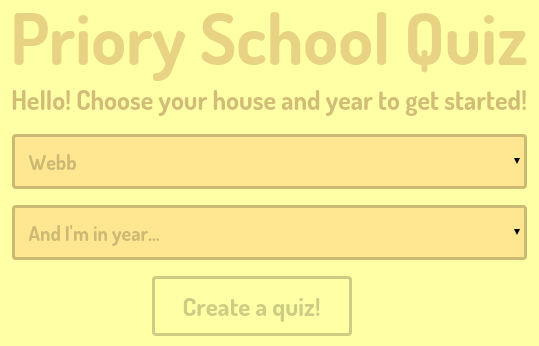
\includegraphics[width=0.95\linewidth]{testing/colours/webb}
  \setcounter{subfigure}{5}%
  \caption{Webb}
  \label{fig:sub2}
\end{subfigure}
\caption{The different house themes.}
\label{fig:test}
\end{figure}
\\As the above images demonstrate, the system correctly themed itself in different colours depending on which houses were chosen. Acton was blue, Baxter orange, Clive a shade of turquiouse, Darwin was purple, Houseman red, and Webb was yellow; all according to the test plan. \textit{Success.}
